\documentclass[border=5]{standalone}
\usepackage{tikz}
\usetikzlibrary{calc}
\begin{document}
	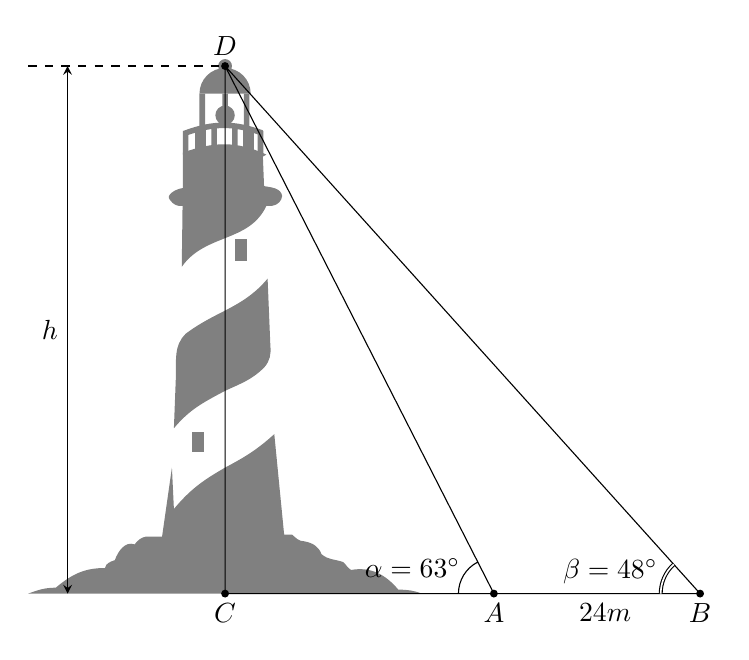
\begin{tikzpicture}[scale=.5,declare function={h=13.4;a=h/tan(63);b=h/tan(48);}]
		\fill[gray] (-5,0) 
		to[out=20,in=180] (-4.3,.15)
		to[out=40,in=180] (-3.05,.65)
		to[out=80,in=200] (-2.8,.85)
		to[out=70,in=160] (-2.3,1.25)
		to[out=50,in=190] (-2,1.45)
		--(-1.6,1.45)--(-1.35,3.2)--(-1.3,2.15)
		to[out=50,in=210] (0,3.2)
		to[out=28,in=222] (1.25,4.05)
		--(1.5,1.5)--(1.7,1.5)
		to[out=-40,in=180] (2,1.33)
		to[out=-10,in=110] (2.45,1)
		to[out=-40,in=160] (3,.8)
		to[out=-40,in=150] (3.2,.6)
		to[out=10,in=130] (4.4,.1)
		to[out=0,in=160] (5,0)
		--cycle;
		\fill[gray] (-.85,3.6) rectangle (-.53,4.1);
		\fill[gray] (-1.3,4.2)
		to[out=50,in=208] (0,5.15)
		to[out=25,in=225] (1,5.75)
		to[out=50,in=275] (1.15,6.3)
		--(1.08,8)
		to[out=-130,in=37] (-1,6.6)
		to[out=-135,in=88] (-1.25,5.5)
		--cycle;
		\fill[gray] (.25,8.45) rectangle (.55,9);
		\fill[gray] (-1.1,8.3)
		to[out=55,in=245] (1.05,9.85)--(1.2,9.85)
		to[out=10,in=263] (1.45,10.1)
		to[out=100,in=-10] (.99,10.35)--(.96,11.1)--(1.05,11.15)
		to[out=155,in=20] (-1.07,11.2)--(-1.07,10.3)
		to[out=-175,in=135] (-1.4,10)
		to[out=-55,in=190] (-1.08,9.85)--cycle;
		\draw[gray,line width= 2pt] 
		(.9,11.15)--(.9,11.75)
		(.25,11.35)--(.25,11.9)
		(-.28,11.35)--(-.28,11.9)
		(-1,11.15)--(-1,11.7)
		to[out=20,in=160] (0.94,11.7)
		(.55,11.8)--(.55,12.7)
		(-.58,11.8)--(-.58,12.7)
		(0,11.9)--(0,12.7);
		\draw[gray,line width=4pt] 
		(.6,11.25)--(.6,11.8)
		(-.63,11.25)--(-.63,11.8);
		\fill[gray] (0,12.15) circle (7pt)
		(.65,12.7) arc (0:180:.65) -- cycle
		(0,13.4) circle (5pt);
		\path 
		(0,0) coordinate (C)
		(a,0) coordinate (A)
		(b,0) coordinate (B)
		(0,h) coordinate (D);
		\foreach \i/\g in {C/-90, A/-90, B/-90, D/90} \fill (\i)circle(.1) node[shift={(\g:.25)}] {$\i$};
		\draw (C)--(B)node[pos=.8, below]{$24m$}--(D)--cycle (A)--(D)
		(A)+(-.9,0) arc (180:117:.9)node[pos=.75, left]{$\alpha=63^\circ$};
		\draw[double] (B)+(-1,0) arc (180:132:1)node[pos=.7, left]{$\beta=48^\circ$};
		\draw[dashed] (-5,h)--(D);
		\draw[stealth-stealth] (-4,0) -- (-4,h)node[pos=.5, left]{$h$};
	\end{tikzpicture}
\end{document}